\documentclass[twocolumn, 8pt]{extarticle}

% Uncomment to squeeze everything onto one side
% \usepackage{pgfpages}
% \pgfpagesuselayout{2 on 1}[letterpaper, landscape]

\usepackage[letterpaper,margin=0.25in]{geometry}
\input{ncommon}
\everymath{}
\usepackage{titlesec}

\titleformat{\section}
  {\normalfont\fontsize{10}{12}\bfseries}{\thesection}{1em}{}
\titlespacing\section{0pt}{4pt plus 2pt minus 2pt}{3pt plus 2pt minus 2pt}
\titlespacing\subsection{0pt}{3pt plus 2pt minus 2pt}{3pt plus 2pt minus 2pt}
\titlespacing\subsubsection{0pt}{3pt plus 2pt minus 2pt}{3pt plus 2pt minus 2pt}
\renewcommand{\arraystretch}{1.5}

\title{ROB310 Midterm Aidsheet}
\author{Tyler Tian}

\begin{document}

\setlength{\abovedisplayskip}{3pt}
\setlength{\belowdisplayskip}{3pt}
\setlength{\parindent}{0pt}

\section{System Modelling} %%%%%%%%%%%%%%%%%%%%%%%%%%%%%%%%%%%%%%%%%%%%%%%%

Continuous time (linear):
$$\begin{aligned} \dot{\bm x}(t) = \bm A\bm x(t) + \bm B\bm u(t), \bm x(0) = \bm x_0 \qquad \bm y(t) = \bm C\bm x(t) + \bm D\bm u(t)\end{aligned}$$
Continuous time (nonlinear):
$$\begin{aligned}\dot{\bm x}(t) = \bm f(\bm x(t), \bm u(t)), \bm x(0) = \bm x_0 \qquad \bm y(t) = \bm h(\bm x(t), \bm u(t))\end{aligned}$$
Discrete time (linear):
$$\begin{aligned}\bm x_{k + 1} = \bm A_d\bm x_k + \bm B_d\bm u_k \qquad \bm y_k = \bm C\bm x_k + \bm D\bm u_k\end{aligned}$$
With a zero-order hold:
\begin{gather*}\mattwo{\bm A_d}{\bm B_d}{\bm 0}{\bm I} = \exp\left(\mattwo{\bm A}{\bm B}{\bm 0}{\bm 0}h\right) \qquad \bm A_d = e^{\bm Ah}, \bm B_d = \int _0^h e^{\bm A\tau'}\dd\tau'\bm B\end{gather*}

\section{Numerical Stability} %%%%%%%%%%%%%%%%%%%%%%%%%%%%%%%%%%%%%%%%%%%%%%%%

Well conditioned problem: $\operatorname{Cond}_x$ small or $\operatorname{cond}_x \leq 1$
\begin{gather*}
\operatorname{Cond}_x = \abs*{\frac{\Delta\bar y}{\Delta x}} \approx \abs*{\diff{f}{x}} \qquad \operatorname{cond}_x = \abs*{\frac{\delta\bar y}{\delta x}} \approx \abs{K_x} = \abs*{\diff{f}{x} \cdot \frac{x}{f(x)}}
\end{gather*}
$\varphi$ is \textit{order} $p$ or $O(\Delta^p)$ if: $\tilde y = \varphi(x, \Delta) - f(x) \propto \Delta^p$

Consistency: $\displaystyle\lim _{\Delta \to 0} \varphi(x, \Delta) = f(x)$ \qquad Stability: $\displaystyle\abs*{\frac{\Delta\tilde y}{\Delta x}} \approx \abs*{\diff{\varphi}{x}} < 1$

$\hat y = \varphi(\hat x, \Delta) = \varphi(\hat x + \Delta x)$ converges to $f(x)$ for $\Delta \to 0$ if it's consistent and at least marginally stable.

$\dot{\bm x} = \bm A\bm x$ well-conditioned/stable when $\Re(\lambda) < 0$ for all $\lambda$.

$\bm x_{k + 1} = \bm A\bm x$ well-conditioned/stable when $\abs{\lambda} < 1$ for all $\lambda$.

\section{Numerical Root Finding} %%%%%%%%%%%%%%%%%%%%%%%%%%%%%%%%%%%%%%%%%%%%%%%%

$f$ is \textit{Lipschitz continuous} if
$$\exists c\text{ s.t. }\forall x, z \in \reals, \abs{f(x) - f(z)} \leq c\abs{x - z}$$
An algorithm has \textit{convergence rate/order} $r$ if:
$\lim _{k \to \infty} \frac{\abs{E_{k + 1}}}{\abs{E_k}^r} = C$

\textbf{Bisection:} order 1; requires continuity; have $l_k, r_k$ such that $\sgn f(l_k) \neq \sgn f(r_k)$, check $c = \frac{l_k + r_k}{2}$ each iteration.

\textbf{Fixed-point Iteration:} order 2 if $g'(x^*) \approx 0$, 1 otherwise; requires update function $g(x^*) = x^*$ for Lipschitz $g$ with $c < 1$ for $x \approx x^*$.
To find $g(x)$, rearrange $f(x^*) = 0$ into the form $x^* = g(x^*)$. Start with guess, update as $x_{k + 1} = g(x_k)$.

\textbf{Newton's Method:} order 2; requires continuous differentiability; equivalent to fixed-point iteration with $g(x) = x - \frac{f(x)}{f'(x)}$.
Start with guess, update as $x_{k + 1} = x_k - \frac{f(x_k)}{f'(x_k)}$. Exact for linear $f$ and suffers for highly nonlinear $f$.

\textbf{Secant Method:} order 1.6; Newton with $f'(x_k) \approx \frac{f(x_k) - f(x_{k - 1})}{x_k - x_{k - 1}}$.

\section{Numerical Integration and Differentiation} %%%%%%%%%%%%%%%%%%%%%%%%%%%%%%%%%%%%%%%%%%%%%%%%

\textbf{Midpoint/Trapezoidal Rule:} order 2, approx. $f$ as const./linear
$$\int _{x_i}^{x_{i + 1}} f(x)\,\dx \approx (x_{i + 1} - x_i) \cdot f\left((x_{i + 1} + x_i)/2\right) \approx (x_{i + 1} - x_i) \cdot \frac{f(x_{i + 1}) + f(x_i)}{2}$$

\textbf{Simpson's Rule:} order 4, approx. $f$ as quadratic
$$(x_{i + 1} - x_i) \cdot \frac{f(x_{i + 1}) + 4f\left((x_{i + 1} + x_i)/2\right) + f(x_i)}{6}$$

\textbf{Differentiation:} Forward (order 1), Backward (1), Centered (2) Difference
$$f'(x) \approx \frac{f(x + \Delta) - f(\Delta)}{\Delta} \approx \frac{f(x) - f(x - \Delta)}{\Delta} \approx \frac{f(x + \Delta) - f(x - \Delta)}{2\Delta}$$

\section{Numerical ODE Solving} %%%%%%%%%%%%%%%%%%%%%%%%%%%%%%%%%%%%%%%%%%%%%%%%

\textbf{Forward Euler's Method:} order 1 (global); explicit; conditionally stable if $\abs{1 + h\lambda} < 1$:
$x_{k + 1} = x_k + hf_k$

\textbf{Backward Euler's Method:} order 1 (global); implicit; conditionally stable if $\abs{1 - h\lambda} > 1$:
$x_{k + 1} = x_k + hf_{k + 1}$

\textbf{Trapezoidal Method:} order 2 (global); implicit; conditionally stable if $\abs*{\frac{1 + \frac{1}{2}h\lambda}{1 - \frac{1}{2}h\lambda}} < 1$:
$x_{k + 1} = x_k + \frac{h}{2}(f_{k + 1} + f_k)$

\textbf{Heun's Method (RK2):} order 2 (global); explicit; conditionally stable if $-4 < 2h\lambda + h^2\lambda^2 < 0$:
$x_{k + 1} = x_k + \frac{h}{2}\left(f(x_k + hf_k) + f_k\right)$

\textbf{Fourth-Order Runge-Kutta (RK4):} order 4 (global); explicit.
\begin{gather*}
    x_{k + 1} = x_k + \frac{h}{6}(k_1 + 2k_2 + 2k_3 + k_4) \\
    \begin{aligned}
        \textstyle k_1 = f(x_k),\quad k_2 = f\left(x_k + \frac{1}{2}hk_1\right) \quad k_3 = f\left(x_k + \frac{1}{2}hk_2\right) \quad k_4 = f(x_k + hk_3)
    \end{aligned}
\end{gather*}

\textit{Time constant:} for $\dot{\bm x} = \bm A\bm x$ with complex eigenvalues $\lambda _i$:
$$\tau _i = \Set{\frac{1}{\abs{\Re(\lambda _i)}}, \frac{2\pi}{\abs{\Im(\lambda _i)}}} \qquad \gamma = \frac{\tau _\text{max}}{\tau _\text{min}} \text{ stiff if } > 10^3$$
Rule of thumb: simulate $T = 5\tau _\text{max}$ if system is stable; use step size $h = \min\Set{\frac{\tau _\text{min}}{10}, \frac{T}{200}}$ or number of steps $k = \max\Set{50\gamma, 200}$;
plot with step size $H = \frac{T}{200} = \frac{\tau _\text{max}}{40}$; for stiff systems use a variable-step solver with initial step $\frac{\tau _\text{min}}{10}$.
Use adaptive step size solvers for stiff problems.

\vspace{-1.0em}
\begin{center}
    \centering
    
\includegraphics[width=0.49\linewidth]{lec7_1.png}
    \hfill
    
\includegraphics[width=0.4\linewidth]{lec8_1.png}
\end{center}
\vspace{-3em}

\section{Optimization} %%%%%%%%%%%%%%%%%%%%%%%%%%%%%%%%%%%%%%%%%%%%%%%%

Formulation: minimize $f(\bm x)$, subject to $\bm g(\bm x) = \bm 0$ (equality constraints) and $\bm h(\bm x) \geq \bm 0$ (inequality constraints); $f: \reals^n \mapsto \reals, \bm g: \reals^n \mapsto \reals^m, \bm h: \reals^n \mapsto \reals^p$.

$\bm x^*$ is a \textit{global minimum} if $\forall \bm x \in \reals^n, f(\bm x^*) \leq f(\bm x)$; \\
or \textit{local minimum} if $\exists \varepsilon > 0\text{ s.t. } \forall \bm x \in \reals^n, \norm{\bm x - \bm x^*}_2 < \varepsilon \implies f(\bm x^*) \leq f(\bm x)$

All minima of $f$ are \textit{stationary points}, where $\del f(\bm x) = \bm 0$; to find the global minimum, check all stationary points and boundaries.
% $$\bm H_f(\bm x) = \matthreeb{\ppdiff{f}{x_1}{x_1}}{\cdots}{\ppdiff{f}{x_1}{x_n}}{\vdots}{\ddots}{\vdots}{\ppdiff{f}{x_n}{x_1}}{\cdots}{\ppdiff{f}{x_n}{x_n}}$$
$$\bm H_f(\bm x) = \operatorname*{matrix} _{i, j} \left[\ppdiff{f}{x_i}{x_j}\right]$$
Local minimum if $\bm H_f(\bm x^*) > 0$, maximum if $\bm H_f < 0$, saddle if $\bm H_f = 0$.

A \textit{feasible point} is any $\bm x$ satisfying all constraints; the \textit{feasible set} contains all feasible points.
A \textit{critical point} is a local maximum, minimum or saddle point in the feasible set.

\textit{Lagrange Multipliers:} for equality constraints $\bm g(\bm x) = \bm 0$:
$$\min _{\bm x, \bm\lambda}\Lambda(\bm x, \bm\lambda) = f(\bm x) - \bm\lambda^T\bm g(\bm x)$$

\textit{Karush-Kuhn-Tucker (KTT) Conditions:} $\bm x^*$ is a critical point when there exists $\bm\lambda \in \reals^m$ and $\bm\mu \in \reals^p$ such that:
\begin{enumerate}
    \itemsep 0pt
	\item Stationarity: $\del f(\bm x^*) - \sum _i \lambda _i\del g_i(\bm x^*) - \sum _j \mu _j\del h_j(\bm x^*) = \bm 0$
	\item Primal feasibility: $\bm g(\bm x^*) = \bm 0$ and $\bm h(\bm x^*) \geq \bm 0$
	\item Complementary slackness: $\forall j, \mu _jh_j(\bm x^*) = 0$
	\item Dual feasibility: $\forall j, \mu _j \geq 0$
\end{enumerate}

$f$ is \textit{convex} if $\bm H_f > 0$ for all $\bm x$, or
$$\forall \bm x_1 \neq \bm x_2, \forall \alpha \in (0, 1), f((1 - \alpha)\bm x_1 + \alpha\bm x_2) \leq (1 - \alpha)f(\bm x_1) + \alpha f(\bm x_2)$$
A set $S$ is \textit{convex} if:
$\forall \bm x, \bm y \in S, \alpha \in [0, 1], \alpha\bm x + (1 - \alpha)\bm y \in S$ \\
or $S = \Set{\bm x | f(\bm x) \leq c}$ for some convex $f(\bm x)$.

If the objective $f$ and feasible set are both convex, the problem is convex and has a unique minimum.

\section{Numerical Optimization Algorithms} %%%%%%%%%%%%%%%%%%%%%%%%%%%%%%%%%%%%%%%%%%%%%%%%

$f$ is \textit{unimodular} over $[a, b]$ if there exists $x^* \in [a, b]$ s.t. $f$ is decreasing over $[a, x^*]$ and increasing over $[x^*, b]$.

\textbf{Golden Section Search:} 1D, unconstrained; order 1; requires unimodularity.
Rescale to $[0, 1]$, choose $x_0 = \alpha, x_1 = 1 - \alpha$ for $0 < \alpha < 1/2$; evaluate $f(x_0), f(x_1)$, discard larger side, rescale and repeat.
Using $1 - \alpha = \frac{1}{2}(\sqrt 5 - 1)$ allows using $x_0$ as the next $x_1$.
\vspace{-0.7em}
\begin{center}
    \centering
    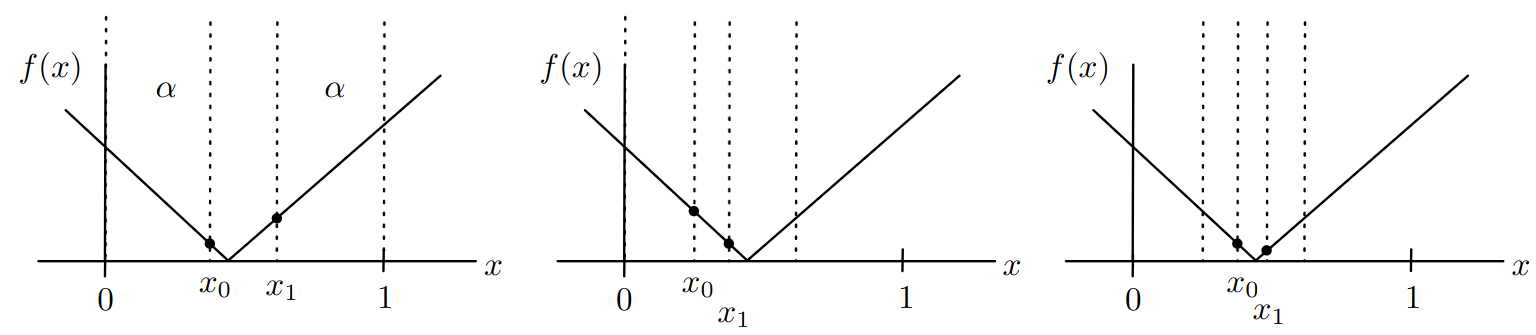
\includegraphics[width=0.8\linewidth]{lec10_1.png}
\end{center}
\vspace{-1em}

\textbf{Gradient Descent:} unconstrained; requires twice differentiable.
Let $g(\alpha) = f(\bm x_k - \alpha\del f(\bm x_k)^T)$, find $\alpha^*$ minimizing $g$, update $x_{k + 1} = x_k - a^*\del f(\bm x_k)^T$.
Optimizing $g$ is expensive so fixed step size can be used. Suffers from poor conditioning of $f$.

\textbf{Newton's Method:} unconstrained; requires twice differentiable.
Iterate as $\bm x_{k + 1} = \bm x_k - \bm H_f^{-1}(\bm x_k)\del f(\bm x_k)^T$; or in 1D, $x_{k + 1} = x_k - \frac{f'(x_k)}{f''(x_k)}$.
Gauss-Newton approximates $\bm H_f$ using first derivatives (mix of gradient descent and Newton).
Levenberg-Marquardt applies adaptive regularization for nearly-singular Hessians.

\textbf{Sequential Quadratic Programming (SQP):} constrained. Iteratively solves a series of simpler, less constrained approximations of the problem.
$f$ is replaced by a quadratic approximation and the constraints linearized. Similar to Newton's method; only converges if initial guess is good.

\textbf{Barrier Methods:} constrained. Constraints are turned into penalties on the objective.
Define new objective as $f'(x) = f(x) + \rho\frac{1}{h(x)}$ where weight $\rho$ is increased to satisfy constraints, decreased for more accuracy.

\section{Linear Algebra} %%%%%%%%%%%%%%%%%%%%%%%%%%%%%%%%%%%%%%%%%%%%%%%%

$\bm A^T\bm A$ is positive definite if $\bm A$ is full rank, semi-definite otherwise.

Orthogonal $\bm Q$ rotates, preserves angles, and $\bm Q^T\bm Q = \bm 1$.

$\bm A\bm x = \bm b$ can be solved by factoring $\bm A = \bm L\bm U$ and solving $\bm L\bm y = \bm b, \bm U\bm x = \bm y$.

A general \textit{vector norm} satisfies: $\norm{\bm x} = 0 \iff \bm x = \bm 0$; $\norm{c\bm x} = \abs{c}\norm{\bm x}$; $\norm{\bm x + \bm y} \leq \norm{\bm x} + \norm{\bm y}$.
The $p$\textit{-norm} for $p \geq 1$ is convex: $$\norm{\bm x}_p = (\abs{x_1}^p + \abs{x_2}^p + \cdots + \abs{x_n}^p)^{\frac{1}{p}}$$
2-norm is Euclidean; $\infty$-norm is $\norm{\bm x}_\infty = \max(\abs{x_1}, \abs{x_2}, \dots, \abs{x_n})$.

The \textit{matrix norm} induced by a vector norm is
$$\norm{\bm A} = \max\Set{\norm{\bm A\bm x} | \norm{\bm x} = 1} = \max _{\bm x \in \reals^n, \bm x \neq 0}\frac{\norm{\bm A\bm x}}{\norm{\bm x}}$$
\textit{1-norm:} max col. sum; \textit{2-norm/spectral radius:} ``largest eigenvalue" of $\bm A$
$$\norm{\bm A}_1 = \max_{i \leq j \leq n} \sum _{i = 1}^m \abs{a_{ij}} \qquad \norm{\bm A}_2 = \max\Set{\sqrt{\lambda} | \exists\bm x \in \reals^n\text{ s.t. }\bm A^T\bm A\bm x = \lambda\bm x}$$
\textit{Frobenius norm:} always $\norm{\bm A}_2 \leq \norm{\bm A}_F$; $\infty$\textit{-norm:} maximum row sum
$$\norm{\bm A}_F = \sqrt{\sum _{i = 1}^m\sum _{j = 1}^n \abs{a_{ij}}^2} = \sqrt{\tr \bm A^T\bm A} \qquad \norm{\bm A}_\infty = \max _{1 \leq i \leq m} \sum _{j = 1}^n \abs{a_{ij}}$$
The \textit{condition number} of $\bm A$ with respect to a norm is $\operatorname{cond} \bm A = \norm{\bm A}\norm{\bm A^{-1}}$
or $\infty$ if $\bm A$ is non-invertible.
For solving $\bm A\bm x = \bm b$, this describes how error in $\bm A$ and $\bm b$ propagates to $\bm x$.

\textbf{Eigendecomposition:} $\bm A = \bm V\bm\Lambda\bm V^{-1}$ where $\bm A\bm v = \bm\lambda\bm v$.

\textbf{Singular Value Decomposition:} $\bm A = \bm U\bm\Sigma\bm V^T$ where $\bm V \in \reals^{n \times n}, \bm U \in \reals^{m \times m}$
are orthogonal, $\bm\Sigma \in \reals^{m \times n}$ is rectangular diagonal with singular values.
Singular values and vectors are related by $\bm A\bm v_i = \sigma _i\bm u _i$.

$\sigma _i = \sqrt{\lambda _i(\bm A^T\bm A)} = \sqrt{\lambda _i(\bm A\bm A^T)}$, total $\max\set{m, n}$ singular values,
nonnegative and real, in decreasing order with $k = \rank\bm A$ nonzero singular values.

$\bm V$ has $k$ eigenvectors of $\bm A^T\bm A$ and $n - k$ orthonormal vectors from $\ker(\bm A^T\bm A)$;
$\bm U$ has $k$ eigenvectors of $\bm A\bm A^T$ and $m - k$ orthonormal vectors from $\ker(\bm A\bm A^T)$.

The rank $j \leq k$ approximation of $\bm A$ is $\sum _{i = 1}^j \sigma _i\bm u_i\bm v_i^T$.

\section{Probability Definitions and Theorems} %%%%%%%%%%%%%%%%%%%%%%%%%%%%%%%%%%%%%%%%%%%%%%%%

The \textit{cumulative distribution function} (CDF) of $f_x(x)$ is $$F_x(x) = \sum _{\bar x = -\infty}^x f_x(x)$$

Given RVs $x \in \mathcal X, y \in \mathcal Y$, \textit{marginalization} (sum rule) and \textit{conditioning}
(product rule) are given by:
$$f_x(x) = \sum _{y \in \mathcal Y} f_{xy}(x, y) \qquad f_{x|y}(x|y) = \frac{f_{xy}(x, y)}{f_y(y)}$$
Which also apply to conditional PDFs; given $z \in \mathcal Z$:
$$f_{x|z}(x|z) = \sum _{y \in \mathcal Y} f_{xy|z}(x, y|z) \qquad f_{x|y,z}(x|y, z) = \frac{f_{xy|z}(x, y|z)}{f_{y|z}(y|z)}$$
The above leads to \textit{total probability theorem} and \textit{Bayes' theorem:}
$$f_x(x) = \sum _{y \in \mathcal Y} f_{x|y}(x|y)f_y(y) \qquad f_{x|y}(x|y) = \frac{f_{y|x}(y|x)f_x(x)}{f_y(y)}$$

$x$ and $y$ are \textit{independent} if $f(x|y) = f(x) \iff f(x, y) = f(x)f(y)$.\\
$x$ and $y$ are \textit{conditionally independent} given $z$ if $$f(x|y, z) = f(x|z) \iff f(x, y|z) = f(x|z)f(y|z)$$

The \textit{expected value} or \textit{mean} of $\bm x$ is
$\displaystyle\bm\mu _x = \mathbb E[\bm x] = \sum _{\bm x \in \mathcal X} \bm xf_x(\bm x)$

The \textit{(co)variance} of $\bm x$ is
$$\bm\Sigma _x = \Var[\bm x] = \mathbb E[(\bm x - \mathbb E[\bm x])(\bm x - \mathbb E[\bm x])^T] = \mathbb E[\bm x\bm x^T] - \mathbb E[\bm x]\mathbb E[\bm x]^T$$
$\Var[x] = \sigma _x^2 = \mathbb E[x^2] - (\mathbb E[x])^2$ in 1D.
$\bm\Sigma$ is symmetric positive (semi-)definite.

\textit{Law of the Unconscious Statistician:} $$\mathcal Y = \Set{y | y = g(x), x \in \mathcal X} \implies \mathbb E[y] = \mathbb E[g(x)]$$

\textbf{Change of Variables:} Given $f_y(y)$, let $x = g(y)$; then
$$\text{Discrete: }f_x(x_j) = \sum _{y_{j,i} \in \mathcal Y_j} f_y(y_{j,i}) \qquad \text{Continuous: }f_x(x) = \frac{1}{\diff{g(y)}{y}}f_y(y)$$
where $\mathcal Y_j$ is the set of all $y_{j,i}$ such that $g(y_{j,i}) = x_j$ (discrete); and $g(y)$ is required to be
continuously differentiable and strictly increasing/decreasing (continuous only).

\section{Bayesian Tracking} %%%%%%%%%%%%%%%%%%%%%%%%%%%%%%%%%%%%%%%%%%%%%%%%

Formulation: computing $f(\bm x_k | \bm y_{1:k})$ from $f(\bm x_{k - 1} | \bm y_{1:k - 1})$, given some motion model
$\bm x_k = \bm f_{k - 1}(\bm x_{k - 1}, \bm v_{k - 1})$ and observation model $\bm y_k = \bm h_k(\bm x_k, \bm w_k)$,
where $\bm x_k, \bm w_k$ are independent with known PDFs, and assuming the \textit{Markov property:}
$f(\bm x_k | \bm x_{k - 1}, \bm x_{k - 2}, \dots) = f(\bm x_k | \bm x_{k - 1})$.

\textbf{Prior Update:} $\displaystyle f(\bm x_k|\bm y_{1:k - 1}) = \sum _{\bm x_{k - 1} \in \mathcal X} f(\bm x_k | \bm x_{k - 1})f(\bm x_{k - 1}|\bm y_{1:k - 1})$

$f(\bm x_k | \bm x_{k - 1})$ can be computed from motion model and noise distribution by change of variables.

\textbf{Measurement Update:} $\displaystyle f(\bm x_k | \bm y_{1:k}) = \frac{f(\bm y_k|\bm x_k)f(\bm x_k|\bm y_{1:k - 1})}{\sum _{\bm \chi_k \in \mathcal X}f(\bm y_k|\bm \chi_k)f(\bm \chi_k|\bm y_{1:k - 1})}$

$f(\bm y_k|\bm x_k)$ can be computed from measurement model and noise distribution by change of variables.
The term in the denominator is for normalization.

\section{Sampling From Distributions} %%%%%%%%%%%%%%%%%%%%%%%%%%%%%%%%%%%%%%%%%%%%%%%%

Given $u$ sampled from $f_u(u)$, a continuous uniform distribution over $(0, 1)$:

\textbf{One Variable, Discrete:} Given a desired PDF $\hat f_x(x)$, remap so $\mathcal X = \integers$, obtain a sample
$x$ by solving $\hat F_x(x - 1) < u \leq \hat F_x(x)$.
\vspace{-0.5em}
\begin{center}
    \centering
    
\includegraphics[width=0.8\linewidth]{lec20_1.png}
\end{center}
\vspace{-1em}

\textbf{One Variable, Continuous:} Obtain sample by $x = \hat F^{-1}(u)$ if CDF is invertible; otherwise pick any $x$
value satisfying $\hat F(x) = u$.

\textbf{Multiple Variables (Finite Sample Space):} Given a desired discrete joint PDF $\hat f_{xy}(x, y)$, let
$\mathcal Z = {1, 2, \dots, N}$ where $N$ is the number of unique combinations of $(x, y)$; define
$\hat f_z(z) = \hat f_{xy}(x, y)$ for some one-to-one mapping $z \leftrightarrow (x, y)$; sample $z$ using the standard
method, then use the mapping to convert to $(x, y)$.

\textbf{Multiple Variables (General):} Find $\hat f_y(y)$ and $\hat f_{xy}(x, y) = \hat f_{x|y}(x|y)\hat f(y)$;
sample $\hat f_y(y)$ for $y$, substitute into $\hat f_{x|y}(x|y)$ to sample for $x$.

\section{Extracting Estimates from PDFs} %%%%%%%%%%%%%%%%%%%%%%%%%%%%%%%%%%%%%%%%%%%%%%%%

Goal: Given observation $\bm y$ and observation model $f(\bm y|\bm x)$, estimate $\bm x$.

\textbf{Maximum Likelihood (ML):} $\displaystyle \hat{\bm x}^\text{ML} = \argmax _{\bm x \in \mathcal X} f(\bm y | \bm x)$ \\
Finds peak of distribution; best used when $f(\bm x)$ is not known. More sensitive to outliers and modelling error,
since the distribution peak might not be the most robust option.

\textbf{Maximum \textit{a Posteriori} (MAP):} $\displaystyle \hat{\bm x}^\text{MAP} = \argmax _{\bm x} f(\bm y | \bm x)f(\bm x)$ \\
Finds peak of distribution $f(\bm x | \bm y)$ given known distribution of $f(\bm x)$. Suffers from the same sensitivity
issues of ML.

\textbf{Minimum Mean Squared Error (MMSE):}
$$\hat{\bm x}^\text{MMSE} = \argmin _{\hat{\bm x}} \mathbb E_{x|y}\left[(\bm x - \hat{\bm x})^T(\bm x - \hat{\bm x})|\bm y\right] = \mathbb E[\bm x|\bm y]$$
Finds expected value/mean of $\bm x$ conditioned on $\bm y$. Typically more robust to outliers and modelling errors as
the entire distribution is considered, but bad for bimodal distributions.

Undesirable cases shown below: Left: ML picks $x_1$, which is not robust. Right: MMSE picks $x_1$, which has zero
probability.
\vspace{-0.5em}
\begin{center}
    \centering
    
\includegraphics[width=0.25\linewidth]{lec21_1.png}
    \qquad
    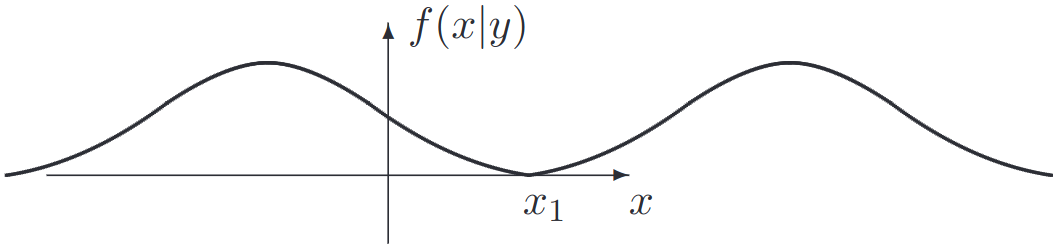
\includegraphics[width=0.5\linewidth]{lec21_2.png}
\end{center}

\section{Properties of Gaussian Distributions} %%%%%%%%%%%%%%%%%%%%%%%%%%%%%%%%%%%%%%%%%%%%%%%%

1-dimensional: $\displaystyle f(x|\mu, \sigma^2) = \frac{1}{\sqrt{2\pi\sigma^2}}\exp\left(-\frac{1}{2}\frac{(x - \mu)^2}{\sigma^2}\right)$

$N$-dimensional: $\displaystyle f(\bm x | \bm\mu, \bm \Sigma) = \frac{1}{\sqrt{(2\pi)^N\det\bm \Sigma}}\exp\left(-\frac{1}{2}(\bm x - \bm\mu)^T\bm \Sigma^{-1}(\bm x - \bm\mu)\right)$

\textbf{Central Limit Theorem:} Let $y_1, \dots, y_n$ be a sequence of $n$ independent random variables drawn from
(possibly different) distributions with finite population mean $\mu$ and variance $\sigma^2$ and let
$\bar y = y_1 + \dots + y_n$, then for $n \to \infty$, $\bar y \sim \mathcal N(n\mu, n\sigma^2)$.

A multivariate Gaussian $\bm x \sim \mathcal N(\bm\mu, \bm\Sigma)$ can be partitioned:
$$\bm x = \cvec{\bm x_1}{\bm x_2}, \bm\mu = \cvec{\bm\mu _1}{\bm\mu _2}, \bm\Sigma = \mattwo{\bm\Sigma _{11}}{\bm\Sigma _{12}}{\bm\Sigma _{21}}{\bm\Sigma _{22}} \implies \bm x \sim f(\bm x_1, \bm x_2)$$
Then $f(\bm x_1) = \mathcal N(\bm\mu _1, \bm\Sigma _{11}), f(\bm x_2) = \mathcal N(\bm\mu _2, \bm\Sigma _{22})$, and
$$f(\bm x_1 | \bm x_2) = \mathcal N(\bm\mu _1 + \bm\Sigma _{12}\bm\Sigma _{22}^{-1}(\bm x_2 - \bm\mu _2), \bm\sigma _{11} - \bm\Sigma _{12}\bm\Sigma _{22}^{-1}\bm\Sigma _{21})$$

Gaussians are preserved in any linear transformation:
\begin{align*}
    &\bm y_1 \sim \mathcal N(\bm a_1, \bm B_1), \bm y_2 \sim \mathcal N(\bm a_2, \bm B_2) \\
    &\qquad\implies \bm C_1\bm y_1 + \bm C_2\bm y_2 \sim \mathcal N(\bm C_1\bm a_1 + \bm C_2\bm a_2, \bm C_1^T\bm B_1\bm C_1 + \bm C_2^T\bm B_2\bm C_2)
\end{align*}
For nonlinear $\bm y = \bm g(\bm x)$, if $\bm x \sim \mathcal N(\bm\mu _x, \bm\Sigma _x)$, then $\bm y \sim \mathcal N(\bm g(\bm\mu _x), \bm A\bm\Sigma _x\bm A^T)$
(approximately) where $\bm A$ is the Jacobian of $\bm g(\bm x)$ at $\bm\mu _x$, if $\bm g$ is roughly linear within
$\pm 3\sigma$ of $\bm\mu _x$. $y \sim \mathcal N(g(\mu _x), a^2\sigma _x^2)$ in 1D where $a = g'(\mu _x)$.

The product of multiple Gaussians is a Gaussian if normalized, with
\begin{align*}
    \mathcal N(\mu, \sigma^2) &= \beta \prod _i \mathcal N(\mu _i, \sigma _i^2)         & \frac{1}{\sigma^2} &= \sum _i \frac{1}{\sigma _i^2}  & \frac{\mu}{\sigma^2} &= \sum _i \frac{\mu _i}{\sigma _i^2} \\
    \mathcal N(\bm\mu, \bm\Sigma) &= \beta\prod _i \mathcal N(\bm\mu _i, \bm\Sigma _i)  & \bm\Sigma^{-1} &= \sum _i \bm\Sigma _i^{-1}          & \bm\Sigma^{-1}\bm\mu &= \sum _i \bm\Sigma _i^{-1}\bm\mu _i \\
\end{align*}

\end{document}
